\documentclass[aspectratio=54,10pt,xcolor=x11names]{beamer}
  \usepackage[french]{babel}
  \usepackage[autolanguage]{numprint}
  \usepackage{fontawesome}
  \usepackage{listings}
  \usepackage[overlay,absolute]{textpos}

  %% =============================
  %%  Informations de publication
  %% =============================
  \renewcommand{\year}{2017}
  \renewcommand{\month}{5}

  %% =======================
  %%  Apparence du document
  %% =======================

  %% Thème de beamer
  \usetheme{metropolis}

  %% Polices de caractères
  % \usepackage{fontspec}
  % \defaultfontfeatures{Ligatures=TeX,Scale=0.88}
  % \setmainfont[Numbers=OldStyle]{Fira Sans}
  %\setsansfont{Lucida Sans OT}
  %\setmathfont{Lucida Bright Math OT}
  % \setmonofont{Inconsolata zi4r Regular}
  % \usepackage[sfdefault,scaled=.88]{FiraSans}
  % \usepackage[varqu,varl]{inconsolata}
  % \usepackage{newtxsf}

  %% Couleurs
  \definecolor{comments}{rgb}{0.7,0,0}  % rouge foncé
  \definecolor{alert}{rgb}{0,0.7,0}     % vert foncé
  \definecolor{link}{rgb}{0,0.4,0.6}    % ~RoyalBlue de dvips
  \definecolor{url}{rgb}{0.6,0,0}       % rouge-brun
  \definecolor{rouge}{rgb}{0.85,0,0.07} % rouge bandeau identitaire
  \definecolor{or}{rgb}{1,0.8,0}        % or bandeau identitaire
  \colorlet{emphasis}{link}
  \colorlet{exercices}{gray}

  %% Hyperliens
  \hypersetup{%
    pdfauthor = {David Beauchemin, Samuel Cabral Cruz, Vincent Goulet},
    pdftitle = {Atelier Introduction à R du colloque R à Québec},
    colorlinks = {true},
    linktocpage = {true},
    allcolors = {link},
    urlcolor = {url},
    pdfpagemode = {UseOutlines},
    pdfstartview = {Fit},
    bookmarksopen = {true},
    bookmarksnumbered = {true},
    bookmarksdepth = {subsection}}

  %% Paramètres de beamer
  % \useinnertheme{default}
  % \useoutertheme[width=10mm,height=2.2\baselineskip]{sidebar}
  % \usefonttheme[onlylarge]{structurebold}
  % \usefonttheme{professionalfonts}
  % \addtobeamertemplate{headline}{\rule{0pt}{12pt}\par}{}
  % \setbeamercolor{frametitle}{fg=white,bg=black}
  % % \setbeamerfont{frametitle}{family=\titles}
  % \setbeamercolor{structure}{fg=emphasis,bg=white}
  % \setbeamercolor{block title}{fg=black,bg=Snow2}
  % \setbeamercolor{alerted text}{fg=black}
  % \setbeamerfont{alerted text}{series=\bfseries}
  % \setbeamercolor{block title alerted}{fg=white,bg=alert}
  % \setbeamercolor{block title example}{fg=white,bg=exercices}
  % \setbeamercolor{example text}{fg=exercices,bg=white}
  % \setbeamertemplate{frametitle continuation}{}
  % \setbeamertemplate{theorems}[numbered]
  % \setbeamertemplate{section in toc}[sections numbered]
  % \setbeamertemplate{navigation symbols}{}
  % \setbeamertemplate{section in sidebar}{}
  % \setbeamertemplate{subsection in sidebar}{}
  % \setbeamertemplate{section in sidebar shaded}{}
  % \setbeamertemplate{subsection in sidebar shaded}{}
  \AtBeginSection[]
  {
    \begin{frame}
      \frametitle{Sommaire}
      \small
      \begin{columns}[t]
        \begin{column}{.5\textwidth}
          \tableofcontents[sections={1-4},%
            currentsection,subsectionstyle=show/show/hide]
        \end{column}
        \begin{column}{.5\textwidth}
          \tableofcontents[sections={5-8},%
            currentsection,subsectionstyle=show/show/hide]
        \end{column}
      \end{columns}
    \end{frame}
  }

  %% Paramétrage de babel pour les guillemets
  \frenchbsetup{og=«, fg=»}

  %% Sections de code source
  \lstloadlanguages{R}
  \lstset{language=R,
    extendedchars=true,
    basicstyle=\small\ttfamily\NoAutoSpacing,
    commentstyle=\color{comments}\slshape,
    keywordstyle=\mdseries,
    showstringspaces=false,
    backgroundcolor=\color{LightYellow1},
    frame=leftline,framerule=1.5pt}


  %% =====================
  %%  Nouvelles commandes
  %% =====================

  %% Noms de fonctions, code, environnement, etc.
  \newcommand{\fichier}[1]{\fbox{\texttt{#1}}}
  \newcommand{\class}[1]{\textbf{#1}}
  \newcommand{\pkg}[1]{\textbf{#1}}
  \newcommand{\link}[2]{\href{#1}{#2~\raisebox{-0.2ex}{\faExternalLink}}}
  \newcommand{\capsule}[2]{\href{#1}{\faYoutubePlay~#2}}

  %% «Bouton» de la page de copyright
  \newcommand{\browsebutton}{%
    \setlength{\fboxrule}{0.5pt}%
    \framebox[20mm][c]{%
      \makebox[2.5mm]{\raisebox{-1pt}{\footnotesize\faGithub}}\;%
      {\sffamily Voir sur GitHub}}}

  %%% =======
  %%%  Varia
  %%% =======

  %% Longueurs pour la composition des pages couvertures avant et
  %% arrière.
  \newlength{\banderougewidth} \newlength{\banderougeheight}
  \newlength{\bandeorwidth}    \newlength{\bandeorheight}
  \newlength{\imageheight}
  \newlength{\logoheight}
  \newlength{\gapwidth}

\begin{document}

\section{Présentation de R}

\begin{frame}
  \frametitle{Bref historique}

  «\emph{R is a free software environment for statistical computing and graphics}»
  \bigskip

  \begin{itemize}
  \item À l'origine fut le S --- milieu des années 1970 --- John~M.\ Chambers
  \item Principalement popularisé par mise en {\oe}uvre commerciale
    S-PLUS
  \end{itemize}
  \bigskip

  \begin{quote}
    \begin{minipage}{0.35\linewidth}
      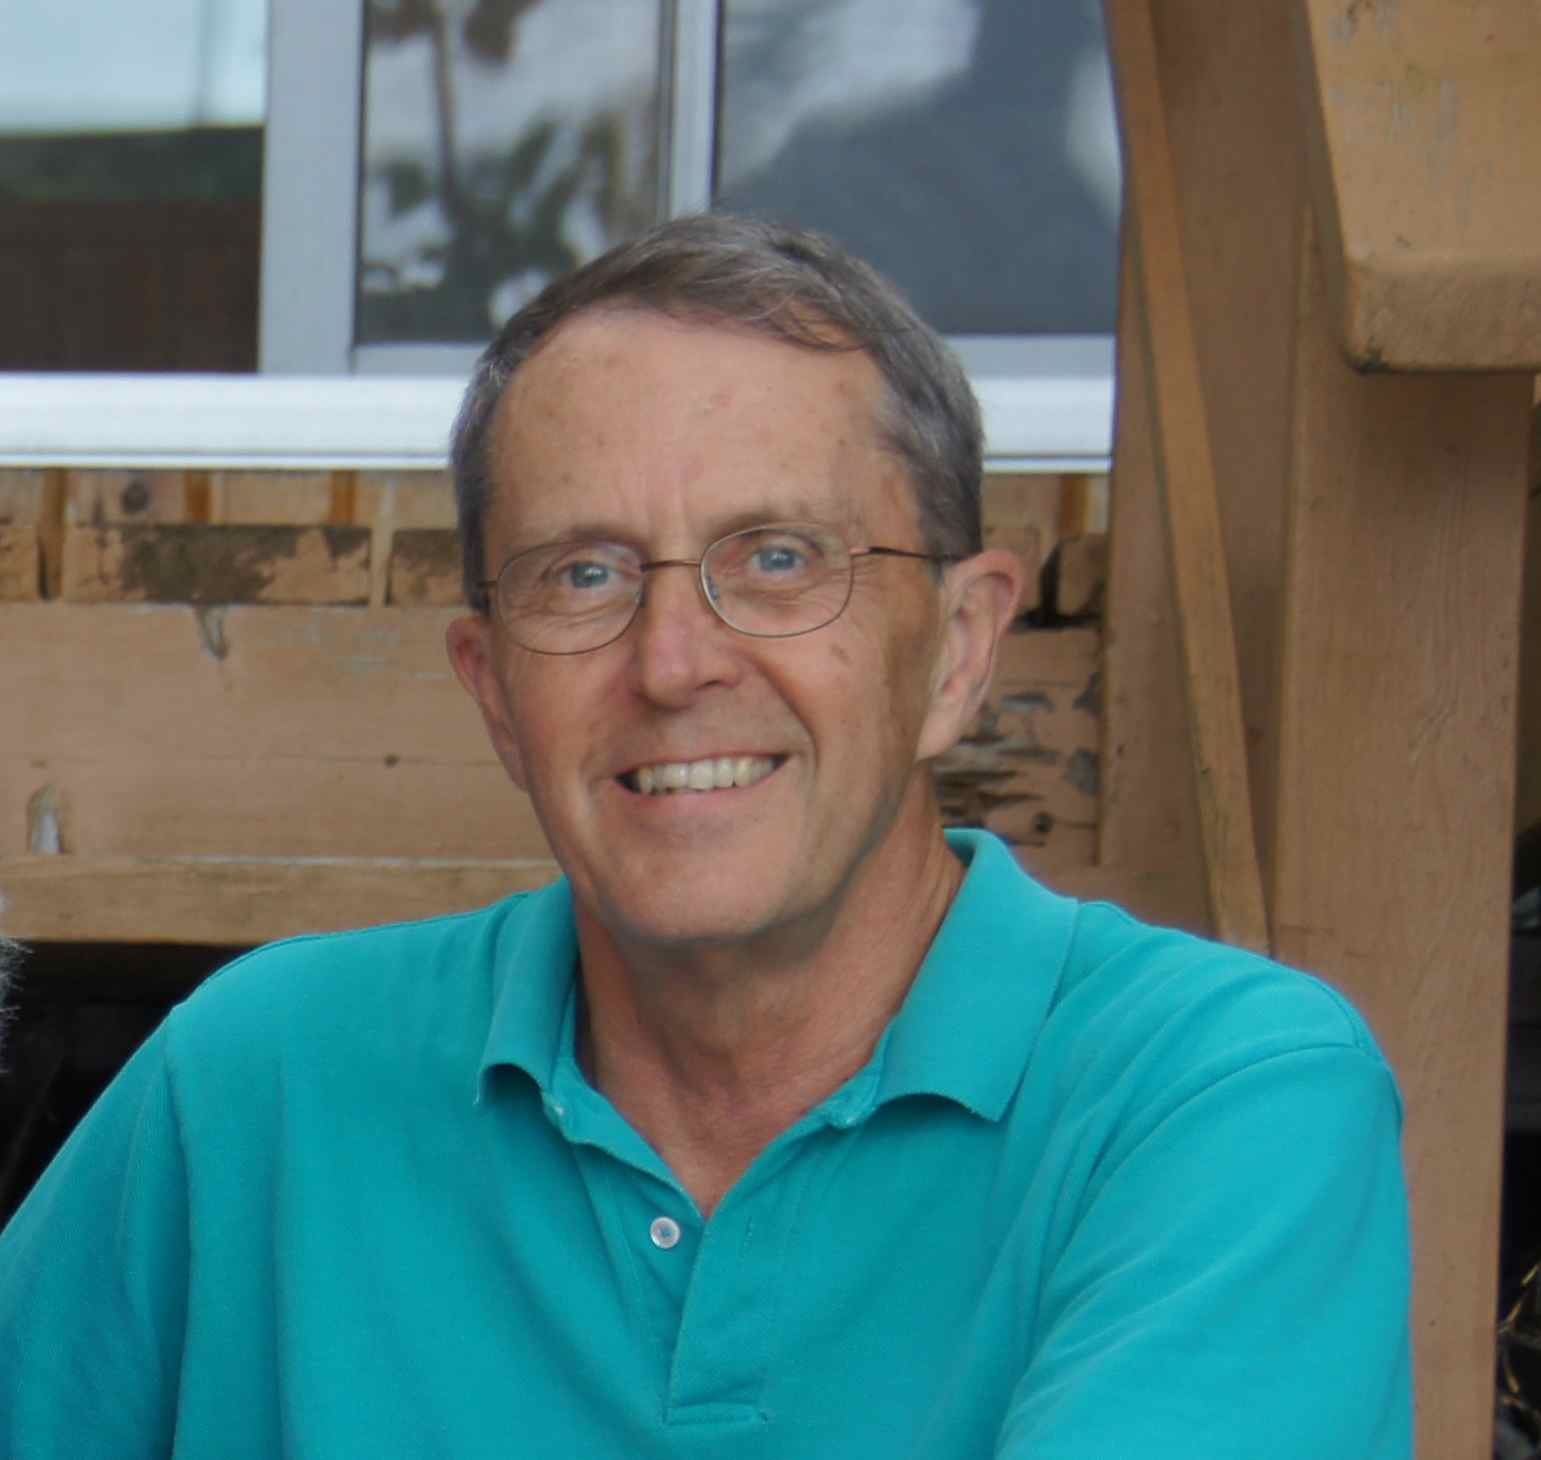
\includegraphics[width=\linewidth,keepaspectratio]{Chambers}
    \end{minipage}
    \hfill
    \begin{minipage}{0.6\linewidth}
      \raggedright
      \textbf{ACM Software System Award 1998} \\
      \emph{John Chambers --- Langage S} \\[\baselineskip]

      «\dots\ which has forever altered how people analyse,
        visualize and manipulate data»
    \end{minipage}
  \end{quote}
\end{frame}

\begin{frame}[fragile=singleslide]
  \frametitle{Bref historique (suite)}

  \begin{itemize}
  \item Nouvelle mise en {\oe}uvre du langage --- milieu des années
    1990 --- \textbf{R}oss Ihaka et \textbf{R}obert Gentleman
  \item Inspirée de Scheme (un dérivé du Lisp) avec syntaxe du S
\begin{Schunk}
\begin{Sinput}
(define factorial (lambda (n)
  (if (= n 1)
      1
    (* n (factorial (- n 1))))))
\end{Sinput}
\end{Schunk}
vs
\begin{Schunk}
\begin{Sinput}
factorial <- function(n)
  if (n == 1) 1 else n * factorial(n - 1)
\end{Sinput}
\end{Schunk}
  \item Libre («GNU S») et ouvert (CRAN) --- R surpasse S-PLUS
  \end{itemize}
\end{frame}

\begin{frame}
  \frametitle{Description sommaire de R}

  \begin{itemize}
  \item Environnement intégré de manipulation de données, de calcul et
    de préparation de graphiques
  \item Aussi un langage de programmation complet
    \begin{itemize}
    \item fonctionnalités statistiques de R programmées en R
    \end{itemize}
  \item Langage \emph{interprété} (et non \emph{compilé})
    \begin{itemize}
    \item analogie avec Excel...
    \end{itemize}
  \end{itemize}

  \begin{center}
    \setlength{\fboxrule}{0.5pt}%
    \href{https://youtu.be/PSQIKSKw_ys}{%
      \framebox[80mm][c]{%
        \makebox[5mm]{\raisebox{-1pt}{\Large\faYoutubePlay}}\;%
        {Principales caractéristiques du langage R}}}
  \end{center}
\end{frame}

\begin{frame}
  \frametitle{Démonstration}
  \begin{itemize}
  \item Interfaces
  \item Stratégies de travail
  \item Éditeurs de texte et environnements intégrés
  \item Anatomie d'une session de travail
  \end{itemize}

  \gotoR{presentation.R}
\end{frame}

%%% Local Variables:
%%% mode: latex
%%% TeX-engine: xetex
%%% TeX-master: "raquebec-atelier-introduction-r"
%%% End:

\include{base}

\end{document}

%%% Local Variables:
%%% mode: latex
%%% TeX-engine: xetex
%%% TeX-master: t
%%% End:
